\section{Konzept}

\subsection{SystemArchitektur}

Dieses Kapitel beschreibt die Erweiterungen und Anpassungen an der Systemarchitektur des bestehenden Praxisrufsystems.
Das System wird um Komponenten zur Signalvermittlung und Sprachsynthese erweitert.
Weiter wird die interne Struktur des Cloudservices angepasst um die Weiterentwicklung und Betrieb des Systems zu optimieren.
\textbf{TODO:} Fix Diagram (Arrows & Names)

\begin{figure}[h]
    \centering
    \begin{minipage}[b]{0.75\textwidth}
        \fbox{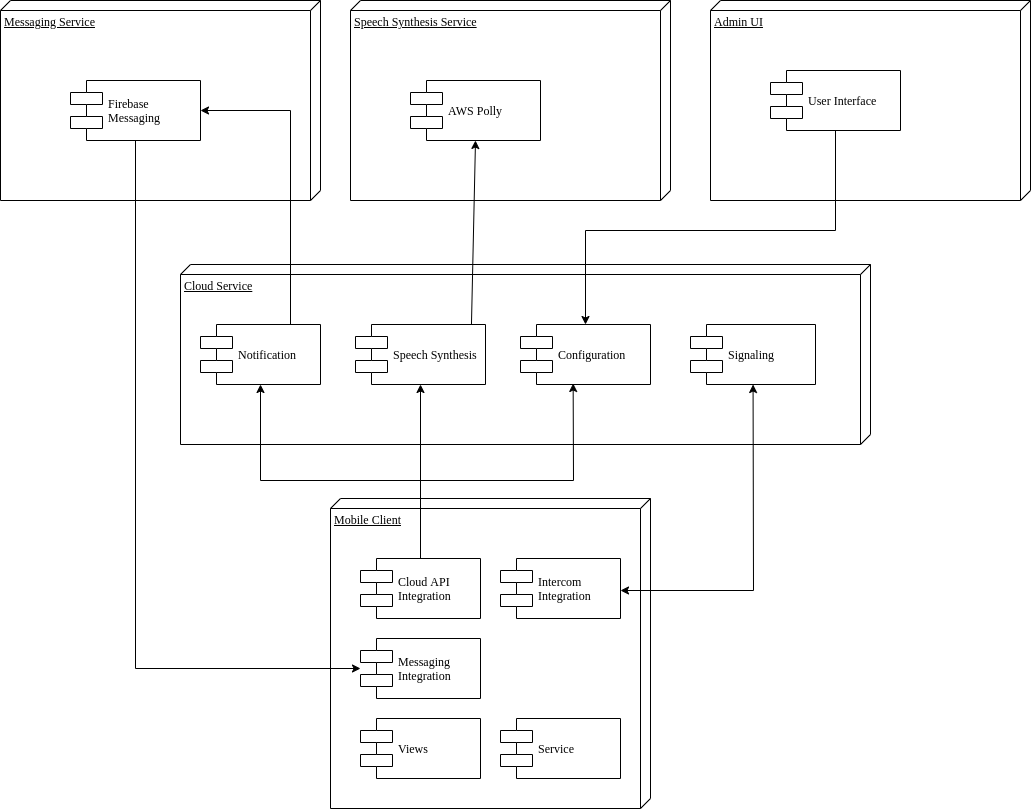
\includegraphics[width=\textwidth]{graphics/diagramms/Component_System_V02}}
        \caption{Systemarchitektur Praxisruf}
    \end{minipage}
\end{figure}

\subsubsection{Systemkomponenten}

Dieses Kapitel gibt eine Übersicht zu den Systemkomponenten von Praxisruf.
Dabei wird für jede Komponente beschrieben, welche Aufgaben ihr zufallen und welche Teile davon mit diesem Projekt angepasst werden.

\textbf{Cloudservice}

Der Cloudservice bildet das zentrale Backend des Praxisruf Systems.
Der Cloudservice wird in die zwei Domänen Notification und Configuration aufgeteilt.
Dabei ist die Domäne Notification für das Versenden von Benachrichtigungen und die Domäne Configuration für die Verwaltung und Auswertung der Konfigurationen verantwortlich.
Zwischen den beiden Domänen besteht eine gerichtete Abhängigkeit.
Die Domäne Notification benötigt zum Versenden von Benachrichtigungen Informationen aus der Configuration Domäne.
Das Identifizieren der relevanten Empfänger geschieht in der Configuration Domäne.
Dementsprechend benötigt die Notification Domäne beim Versenden die Information, an welche Empfänger die Benachrichtigung versendet werden soll.

Die Domänentrennung innerhalb des Cloudservices findet bis heute lediglich auf Package-Ebene statt.
Mit diesem Projekt soll die Trennung einen Schritt weiter gehen.
Die Applikation wird in mehrere Module aufgeteilt.\footnote{Siehe Kapitel 5.1.2}
Diese können zu einem späteren Zeitpunkt in einzelne Microservices aufgeteilt werden.

Nachdem die Auftrennung in Module statgefunden hat, wird der Cloudservice um zwei Module erweitert.
Das neue Modul Signaling ist für die Signalvermittlung zwischen Mobile Clients verantwortlich.
Dies ist nötigt um Peer To Peer Sprachverbindungen zwischen Mobile Clients aufzubauen.
Das Modul Signaling hat eine gerichtete Abhängigkeit zum Module Notification.
Über das Notification Modul sollen Mobile Clients informiert werden, wenn ein Signal nicht versendet werden konnte, weil sie nicht mit dem Cloudservice verbunden waren.
Das neue Modul Speech Synthesis dient als einheitliche Schnittstelle zu einem externen Seepch Synthesis Service.
Dadurch kann auch wenn ein Android oder Web Client kommt, dieser genau gleich angebunden werden.
Garantie, dass die Konfiguration und Funktionsweise dieselbe für alle Clients ist. \\

\textbf{Mobile Client}

Mit dem Vorgängerprojekt wurde bereits ein Mobile Client umgesetzt.
Dieser wurde als Shared Platform Applikation mit Nativescript umgesetzt.
Er bietet Praxismitarbeitenden die Möglichkeit Benachrichtigungen zu versenden und zu empfangen.
Mit diesem Projekt wird der Mobile Client als native iOS Applikation komplett neugeschrieben.
Der neue iOS Client muss sämtliche Funktionen des bestehenden Mobile Clients unterstützen.
Zudem wird im neuen Client die Funktion der Gegensprechanlage und das Vorlesen von Benachrichtigungen über Sprachsynthese umgesetzt.

\textbf{Admin UI}

Das Admin UI ermöglicht dem Praxisadministrator, die Konfiguration des Systems zu verwalten.
Die Konfiguration des Systems wird mit diesem Projekt erweitert.
Einerseits können neu Buttons für die Gegensprechanalge konfiguriert werden.
Andererseits kann eingestellt werden, welche Benachrichtigungen vorgelesen werden sollen.
Beide Informationen müssen über das Admin UI verwaltet werden können.

\textbf{Messaging Service}

Der Messaging Service ist für die Zustellung von Push Benachrichtigungen an Mobile Clients verantwortlich.
Der Cloudservice muss an den Messaging Service angebunden sein, um Benachrichtigungen anhnd der Konfiguration zu versenden.
Die Anbindung des Cloudservices an den Messaging Service ist mit dem Vorgängerprojekt bereits umgesetzt und muss für dieses Projekt nicht angepasst werden.
Der neu entwickelte native Mobile Client muss mit diesem Projekt an den Messaging Service angebunden werden, um Benachrichtigungen zu empfangen.
Als Messaging Service wird Firebase Cloud Messaging verwendet.\\

\textbf{Speech Synthesis Service}

Um Sprach Synthese zu ermöglichen, wird ein externer Service angebunden.
Dieser übernimmt die Konvertierung von Text aus Benachrichtigungen zu synthetisierter Sprache.
Die Anbindung an den Speech Synthesis Service wird ausschliesslich im Cloudservice implementiert.
Sämtliche andere Komponenten die Sprachdaten benötigen, fragen diese beim Cloudservice ab.
Welcher die Abfrage an den Speech Synthesis Service übernimmt und die Resultate dem Anfrager zur Verfügung stellt.
Als Speech Synthesis Service wird Amazon Polly verwendet.

\clearpage

\subsubsection{Modularisierung CloudService}

Mit dem Projekt IP5 Cloudbasiertes Praxisrufsystem wurde der Cloudservice implementiert.
Der Cloudservice trennt intern die beiden Domänen Notification und Configuration.
Die Domäne Configuration ist für die Verwaltung und Auswertung der Konfiguration des Systems verantwortlich.
Die Domäne Notification ist für das Versenden von Benachrichtigungen verantwortlich.
Für das Versenden von Benachrichtigungen werden in der Notification Domäne Informationen aus der Configuration Domäne benötigt.
Diese Informationen werden über eine REST-Schnittstelle abgefragt.

Die Trennung der Notification und Configuration Domänen, ermöglicht es die beiden Teile der Applikation in separaten Services zu betreiben.
So können diese unabhängig voneinander betrieben und erweitert werden.
Weiter wird es dadurch möglich, einzelnen Teilen der Applikation mehr Ressourcen zuzuteilen.
Die Trennung der beiden Domänen in eigene Microservices wurde mit dem Projekt IP5 noch nicht vorgenommen.
Die beiden Domänen wurden lediglich durch die Package Struktur innerhalb eines einzelnen monolithischen Services getrennt.
Mit diesem Projekt soll die Trennung der Domänen einen Schritt weiter vorangetrieben werden.

Neu soll es pro Domäne ein Gradle Modul geben, welches sämtliche Domänenobjekte, Services und Schnittstellen der jeweiligen Domäne kapselt.
Dadurch ist garantiert, dass die Domänen sauber voneinander getrennt sind.
Sämtliche Kommunikation zwischen den Modulen muss über REST-Schnittstellen geschehen.

Um den Betrieb des Cloudservices für dieses Projekt möglichst simpel zu halten, werden die einzelnen Teile immer noch als monolithische Applikation gestartet.
Dazu wird ein Modul \textbf{App} erstellt, welches alle Domänen Module kapselt und in einer Applikation startet.
Um die Applikation zukünftig in einzelne Micro Services aufzutrennen, müssen die einzelnen Module um eine Klasse erweitert werden, welche nur dieses Modul als Applikation startet.
Komponenten, welche in mehr als einer Domäne verwendet werden, werden in ein zusätzliches \textbf{Commons} Modul verlegt.
Dazu gehören Data Transfer Objects für Schnittstellen zwischen den Modulen, geteilte Clients um Abfragen auf andere Module abzusetzen sowie Komponenten für Security und Fehlerhandling.
Neben den Modulen App und Commons, werden vier weitere Module für die Domänen Configuration, Notification, Speech Synthesis und Signaling erstellt.
Das Modul \textbf{Configuration} beinhaltet alle Domänenobjekte, Services und Schnittstellen für die Verwaltung, Auswertung und Abfrage der Systemkonfiguration.
Das Modul \textbf{Notification} beinhaltet alle Domänenobjekte, Services und Schnittstellen für das Versenden von Benachrichtiungen.
Das Modul \textbf{Speech Synthesis} beinhaltet die Anbindung an den Speech Synthesis Service und stellt eine Schnittstelle zur verfügung über den das restliche System Sprachdaten beziehen kann.
Das Modul \textbf{Signaling} beinhaltet Domänenobjekte, Services und Schnittstellen für die Signalgvermittlung zwischen Mobile Clients.

\clearpage
